\section{Simulation Analysis}
\label{sec:simulation} 
For the simulation we simplified the script by using an independent sinusoidal power source that matches the secondary coil of the inductor, corresponding to a ratio n of $n=1/12.665565 = 0.078954235$
\par In these section we represent the plots that were produced by doing operating point using Ngspice. These plots represents the Voltage on Envelope Detector and the output voltage of the circuit.


\begin{figure} [!htb] 
  \minipage{0.9\textwidth}
  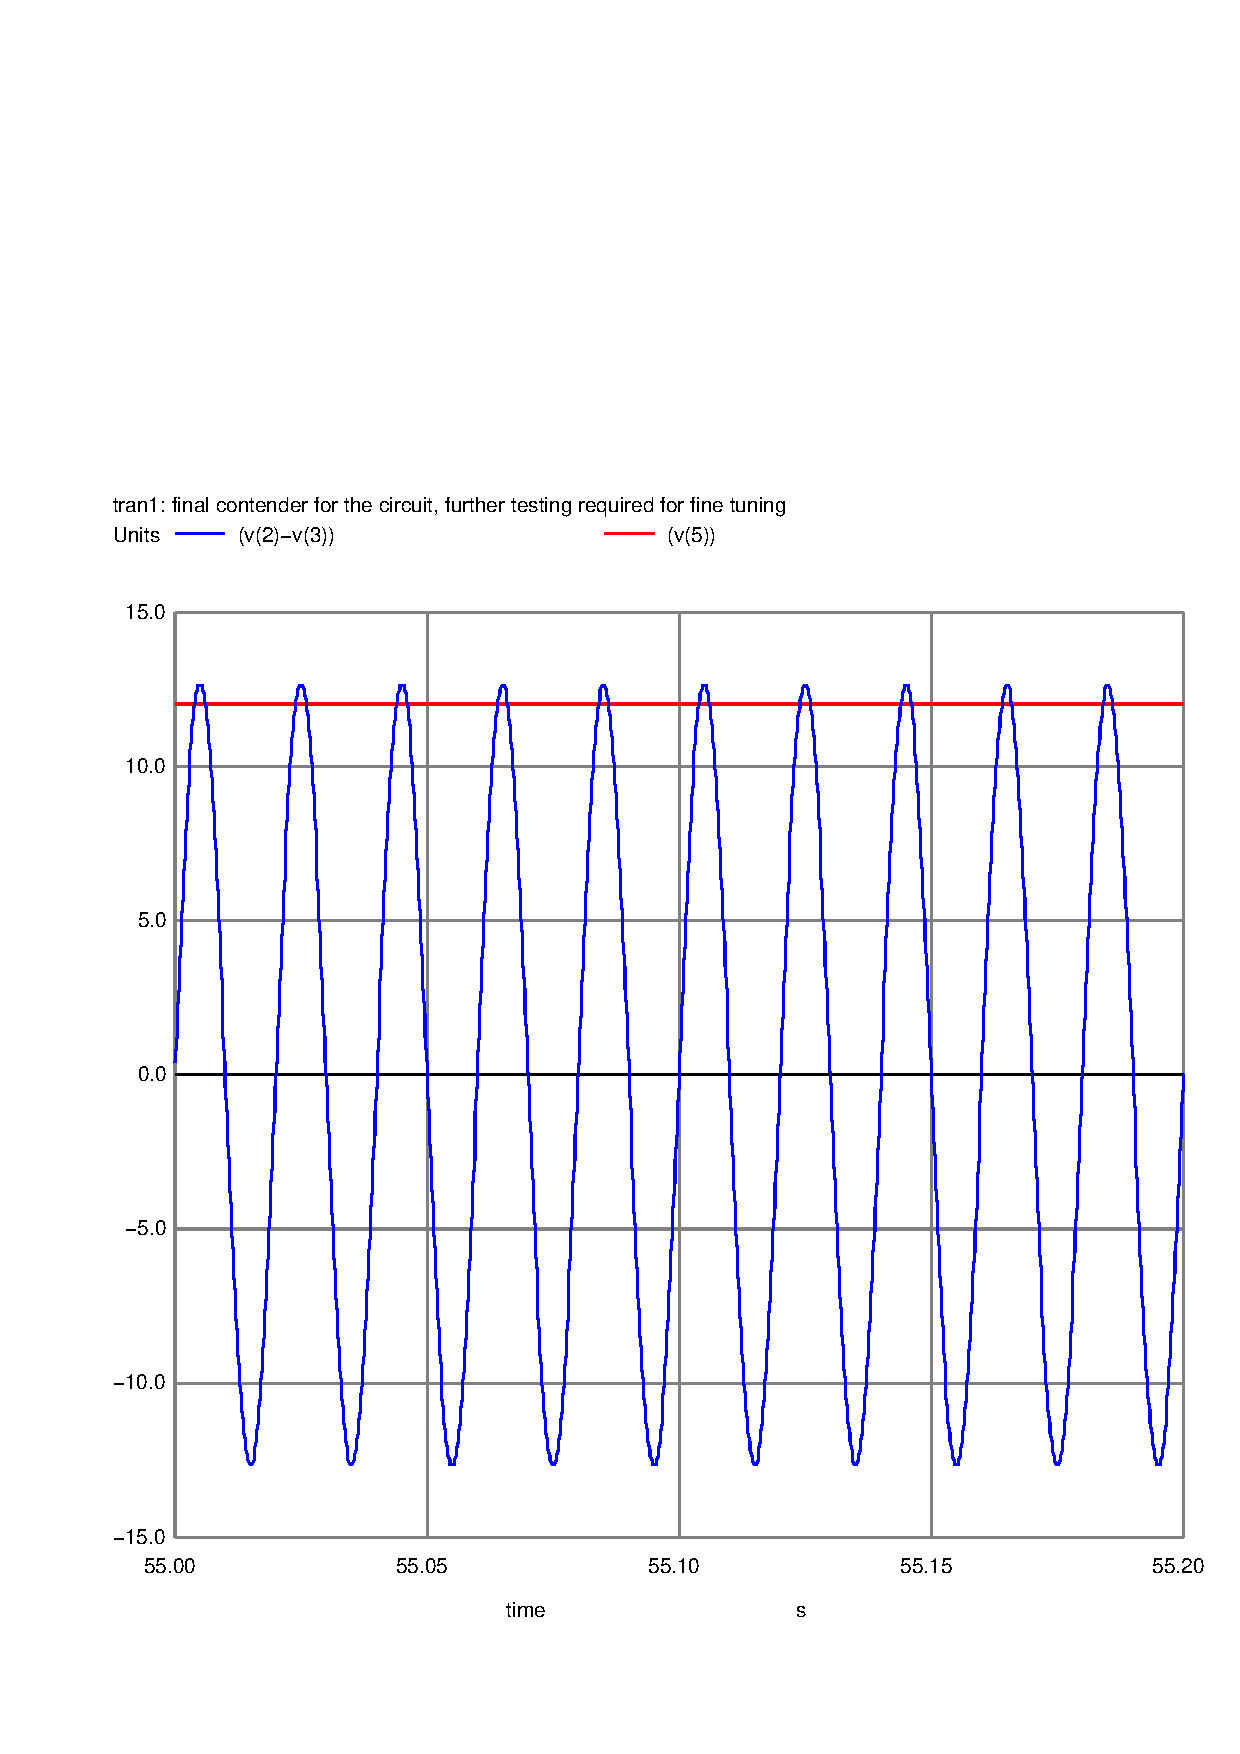
\includegraphics[width=\linewidth]{out.pdf}
  \caption{Envelope Detector and Output Voltages}
  \label{fig:theoplots}
  \endminipage\hfill
\end{figure}



\begin{figure} [!htb]
  \minipage{0.9\textwidth}
  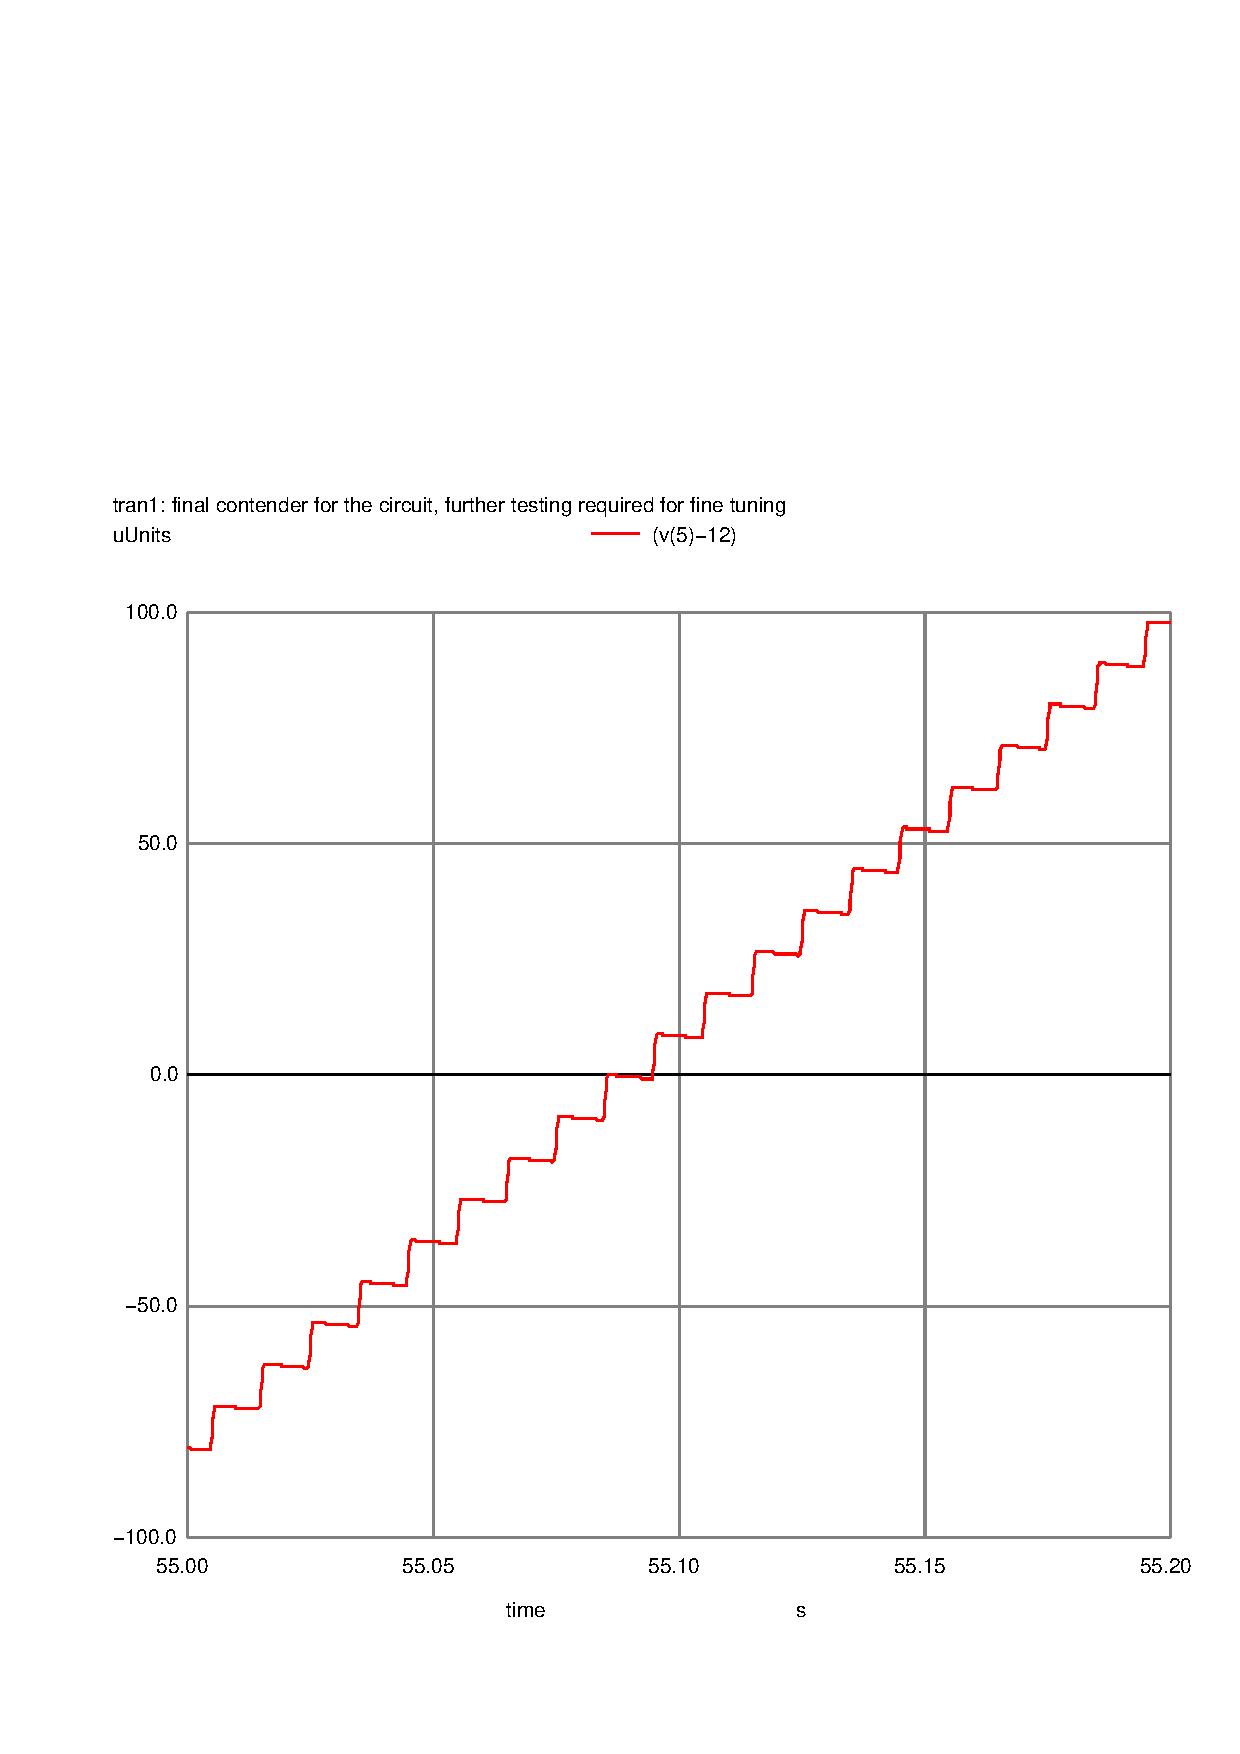
\includegraphics[width=\linewidth]{zoom.pdf}
  \caption{Output AC component + DC deviation}
  \label{fig:theoplots}
  \endminipage\hfill
\end{figure}


\par And finally, we have computed the results of the voltage ripple and the output DC level.  

\FloatBarrier
\begin{table}[h]
  \centering
  \begin{tabular}{|c|c|c|}
    \hline    
    maximum(v(5)) & 1.200010e+01\\ \hline
minimum(v(5)) & 1.199992e+01\\ \hline
mean(v(5)) & 1.200001e+01\\ \hline

    \hline
  \end{tabular}
  \caption{Voltages}
  \label{tab:Spice1}
\end{table}
\FloatBarrier  

\FloatBarrier
\begin{table}[h]
  \centering
  \begin{tabular}{|c|c|c|}
    \hline    
    maximum(v(5))-minimum(v(5)) & 1.791424e-04\\ \hline
mean(v(5)-12) & 8.510638e-06\\ \hline

    \hline
  \end{tabular}
  \caption{Ripple an mean DC deviation}
  \label{tab:Spice2}
\end{table}
\FloatBarrier 

From this table we can take the ripple voltage value $V_{ripple}=maximum(v(5))-minimum(v(5))$ and also the value of the DC level, $mean(v(5))$ and corresponding deviation from the target of 12V.\\
Combined with a cost of 74.2 this gave us the merit that can be seen in the following line.


\FloatBarrier
\begin{table}[h]
  \centering
  \begin{tabular}{|c|c|c|}
    \hline    
    1/ (74.2* ((maximum(v(5))-minimum(v(5))) + mean(v(5)-12) + 1e-6)) & 7.143848e+01\\ \hline

    \hline
  \end{tabular}
  \caption{Merit figure}
  \label{tab:Spice2}
\end{table}
\FloatBarrier 
